\pagestyle{empty}
\begin{titlepage} %Esta es la caratula
	
\centering
{Instituto Tecnológico de Buenos Aires \par}
\vspace{2cm}

{\scshape \Huge \bf Elementos Finitos\par}

\vspace{.8cm}

{\scshape\Large Apunte no oficial para la materia 30.07 y 31.92 \par}
\vfill
\vspace{3cm}

{
	\centering
	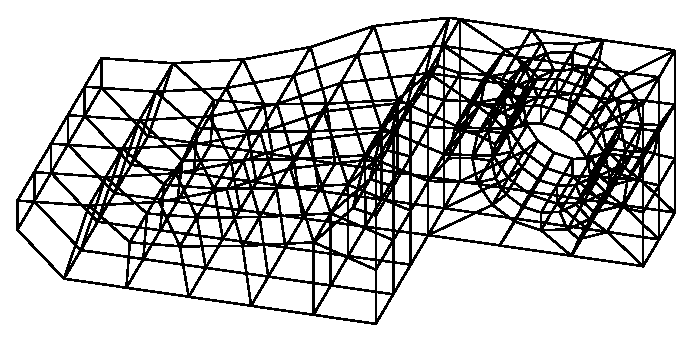
\includegraphics[width=\textwidth]{fig/sear.eps}
	
}
\vfill

{\scshape\Large\textbf{Patricio Whittingslow} \par}
\vspace{4cm}
\medskip %medskip,smallskip,vspace son todos comandos para dejar espacio en blanco entre cosas

\end{titlepage} %Termina la caratula
\pagestyle{plain}